With the analytical models developed in the previous sections, now we compare the energy savings among different fault tolerance approaches, i.e., lazy shadowing, stretched replication, and state machine replication. Without loss of generality, we assume the maximal execution rate is normalized such that $\sigma_{max}=1$. The derived optimal execution rates are presented as fractions of the maximal execution rate. 

During the experiments, we identified several critical parameters in the analytical models, which represents the characteristics of the task, and the underlying system. These parameters include:
\begin{itemize}
	\item $\rho$ -- static power ratio, which determines how much power consumption is independent of the execution rate.
	\item $W$ -- workload of the task.
	\item MTBF -- the reliability of the system that runs the task.
	\item $\alpha$ -- the laxity in the response time that can be tolerated.
\end{itemize}
In the following, we will present our sensitivity study results with respect to the above parameters. In each of the sensitivity study, we normalize the energy consumption of lazy shadowing and stretched replication to that of state machine replication. 

\subsection{Response time laxity}
Response time is always an important factor to consider in HPC as system efficiency is critical and high throughput is desirable. In the experiments we find that the energy savings of lazy shadowing and stretched replication versus traditional replication are largely impacted by the laxity in response time. This is mainly due to the fact that both of the proposed approaches rely on reducing the execution rates to save energy, while the laxity in response time determines how much the execution rate can be reduced. The results for $W=240$ hours and MTBF=5 years are shown in Figure~\ref{fig:alpha}. Two values for $\rho$ are used.

\begin{figure}[!t]	
	\begin{center}
		\subfigure[$\rho=0.5$]
		{
			\label{fig:alpha_1}
			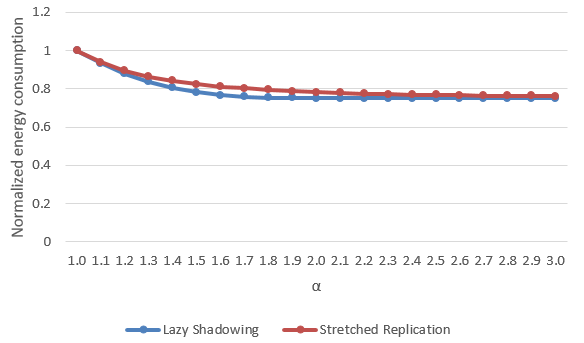
\includegraphics[width=\columnwidth]{figures/alpha_1.png}
		}
		\subfigure[$\rho=0.3$]
		{
			\label{fig:alpha_2}
			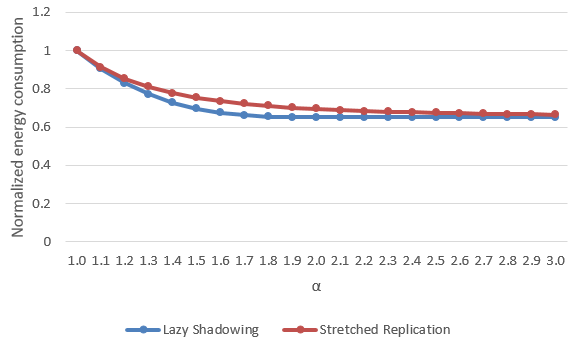
\includegraphics[width=\columnwidth]{figures/alpha_2.png}
		}
	\end{center}
	\caption{Energy consumption comparison for various response time laxity. W=240 hours, MTBF=5 years.}
	\label{fig:alpha}
\end{figure}


Figure~\ref{fig:alpha} shows that both lazy shadowing and stretched replication can achive over 20\% of energy savings compared to state machine repilcation, when there is enough laxity in the response time. When there is no laxity in the response time ($\alpha=1$), lazy shadowing and stretched replication don't have any freedom to reduce the execution rate of the shadow process, thus will execute both the main and shadow processes at the maximal execution rate, which essentially converges to state machine replication. In this case, it is staightforward that all three approaches have the same energy consumption. However, as laxity in response time increases, lazy shadowing and stretched replication immediately gain the ability to slow down the shadow process and thus save energy. It is also clear that laxy shadowing has more potential than stretched replication in energy saving. It can take better advantage of the laxity in respone time as it is more flexible in controling the execution rate than stretched replication. The highest difference is 4.5\% when $\alpha$ is around 1.5. As the laxity keeps increasing, the energy savings by lazy shadowing and stretched replication flatten out, as a result of the static power consumption. Since the static power consumption is independent of the execution rate, reducing the execution rate would extend the execution time, resulting in an increase in the energy consumption corresponding to the static power. Therefore, the minimal energy consumption would be achieved when there is a balance between energy from dynamic power and energy from static power, which may not be necessarily equivalent to using all the laxity in response time. It can be projected that if the staic power ratio is lower, laxy shadowing and stretched replication can take advantage of more laxity and achieve more energy saving compared to state machine replication. This will be discussed further in later section. At the right side of Figure~\ref{fig:alpha_1} and Figure~\ref{fig:alpha_2}, lazy shadowing and stretched replication converge when there is enough laxity for both of them. 

\subsection{Task vulnerability}
The objective of lazy shadowing is to minimize the expected energy consumption, considering the characteristics of both the task to execute and the underlying system. The probability of failure during the execution of the task is an important factor that will impact how the proposed fault tolerance approaches execute the task. Specifically, they will choose different process execution rates according to the likelyhood of failures. The ratio between the task workload and the MTBF is an approximation of the likelyhood of failure, assuming task workload is far less than the MTBF. In our experiments, we find that there is a linear relationship between task workload and MTBF in determining the optimal execution rates. Specifically, increasing the task workload has the same effect as decreasing the MTBF in our analytical models. Therefore, we combine them as a single parameter and refer to it as task vulnerability.

\begin{figure}[!t]	
	\begin{center}
		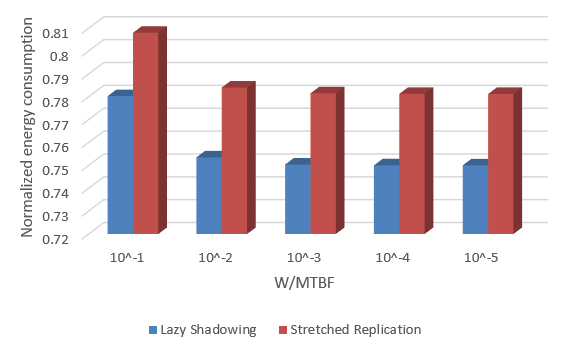
\includegraphics[width=\columnwidth]{figures/vulnerability.png}
	\end{center}
	\caption{Energy consumption consumption for various task vulnerabilities. W=240 hours, $\rho$=0.5.}
	\label{fig:vulnerability}
\end{figure}

The results of the sensitivity study to task vulnerability, when $W=240$ hours and $\rho=0.5$, are shown in Figure~\ref{fig:vulnerability}. From left to right, the task vulnerability decreases, meaning that the likelyhood of failure decreases. We can see that for all task vulnerabilities considered, both lazy shadowing and stretched replication can achieve significant energy savings over state machine replication. This indicates that the proposed approaches are scalable to future large-scale and failure-prone HPC environments. As task vulnerability decreases, lazy shadowing and stretched replication gains more energy savings. This is because the probability that the main process can complete the task without failure increases when task vulnerability decreases, increasing the probability that the shadow process can be terminated early to save energy. Again, lazy shadowing outperforms stretched replication because of its more flexibility in controling the execution rate of its shadow process.

\subsection{Static power ratio}
The computing nodes of each supercomputers have different power consumption characteristics, depending on the various computer organization and architecture technologies. Since our approaches are based on DVFS to control the process execution rates, the power consumption is partitioned into dynamic power, which has a superlinear relationship with the execution rate, and static power, which is unaffected by the execution rate. Static power ratio is an effecitve way to abstract the power saving ability of the proposed approaches on different machines.

\begin{figure}[!t]	
	\begin{center}
		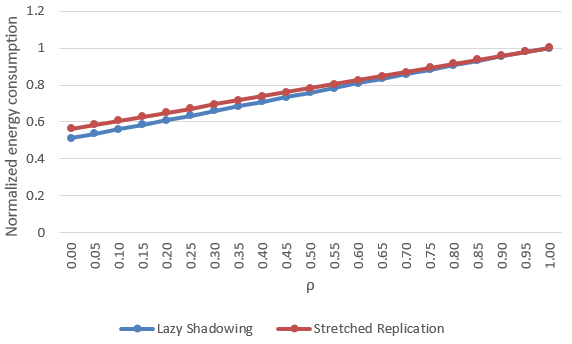
\includegraphics[width=\columnwidth]{figures/rho.png}
	\end{center}
	\caption{Energy consumption consumption for various static power ratios. W=240 hours, $\alpha$=2, MTBF=5 years.}
	\label{fig:rho}
\end{figure}

DVFS saves dynamic power while not changing static power. These two aspects have conflicting effects on the total energy consumption. By reducing the execution rate, the execution time increases proportionally. This also increases the energy consumption from static power proportionally as the static power is constant. However, since the dynamic power can be reduced superlinearly, the energy consumption corresponding to dynamic power is reduced, even though the execution is extended. The above analysis can be illustrated with Figure~\ref{fig:rho}. In addition, Figure~\ref{fig:rho} reveals that lazy shadowing can save up to 49\% of energy over state machine replication when consider dynamic power only. On the other hand, lazy shadowing and stretched replication are forced to execute both the main and shadow processes at the maximal rate when dynamic power is negligible, converging to the behavior of state machine replication. Current supercomputers have a static power ratio between 40\%-70\%, and it is reasonable to suspect that this will continue to be the case. Within this range, the energy saving is 14\%-29\% for lazy shadowing, and 13\%-26\% for stretched replication.

